% !TeX spellcheck = en_US
\documentclass[french]{yLectureNote}

\title{Mécanique 2}
\subtitle{Chimie}
\author{Paulhenry Saux}
\date{\today}
\yLanguage{Français}

\professor{IHallery}%isabelle.hallery@univ-tlse3.fr
\usepackage{graphicx}%----pour mettre des images
\usepackage[utf8]{inputenc}%---encodage
\usepackage{geometry}%---pour modifier les tailles et mettre a4paper
%\usepackage{awesomebox}%---pour les boites d'exercices, de pbq et de croquis ---d\'esactiv\'e pour les TP de PC
\usepackage{tikz}%---pour deiffner + d\'ependance de chemfig
% \usepackage{tabularx}%---pour dimensionner automatiquement les tableaux avec variable X
\usepackage{awesomebox}%---Pour les boites info, danger et autres
\usepackage{menukeys}%---Pour deiffner les touches de Calculatrice
\usepackage{fancyhdr}%---pour les en-t\^ete personnalis\'ees
\usepackage{blindtext}%---pour les liens
\usepackage{hyperref}%---pour les liens (\`a mettre en dernier)
\usepackage{caption}%---pour la francisation de la l\'egende table vers Tableau
\usepackage{pifont}
\usepackage{array}%---pour les tableaux
\usepackage{lipsum}
\usepackage{yFlatTable}
\usepackage{multicol}
\newcommand{\Lim}[1]{\lim\limits_{\substack{#1}}\:}
\renewcommand{\vec}{\overrightarrow}
\newcommand{\N}[0]{\mathbb{N}}
\newcommand{\dd}{\mathrm{d}}
\newcommand{\norm}[1]{||\vec{#1}||}
\begin{document}
\chapter{Repérage}
\section{Repérage}
\subsection{introduction}
On utilise un repère définit par
\begin{itemize}
    \item une origine
    \item 3 vecteurs unitaires formant une base orthonormé directe (le produit vectoriel des 2 premiers vaut le 3e vecteur)
\end{itemize}
\subsection{Système cylindrique local}
\begin{multicols}{2}
3 vecteurs unitaires :
\begin{itemize}
 \item $\vec{e_{\rho}}$ appelé vecteur radial
  \item $\vec{e_{\varphi}}$ appelé vecteur orthoradial
  \item $\vec{e_z}$
\end{itemize}

\subsubsection{Coordonnées cartésiennes en fonction des cylindriques}
\begin{itemize}
 \item $x = \rho \cos(\varphi)$
 \item $ y = \rho \sin(\varphi)$
 \item $z = z$
\end{itemize}
\columnbreak

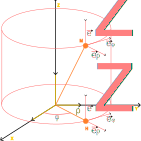
\includegraphics[scale=0.5]{base_c}

\end{multicols}
\subsubsection{Coordonnées cylindriques en fonction des cartésiennes}
\begin{itemize}
 \item $\rho = \sqrt{x^2+y^2}$
 \item $\varphi = \tan^{-1}(\frac{y}{x}) = \cos^{-1}(\frac{x}{\sqrt{x^2+y^2}}) = \sin^{-1}(\frac{y}{\sqrt{x^2+y^2}})$
%  \marginCritical{Attention aux conditions pour utiliser ces formules : celle avec $\tan^{-1}$ nécessite que y et x soient positifs (dans le cas contraire, il faut rajouter $\pi$) et celle avec $\cos^{-1}$ que y soit positif.}
\end{itemize}

\subsubsection{Relation entre les vecteurs}
\begin{itemize}
 \item $\vec{e_{\rho}} = \cos( \varphi) \vec{e_x}+\sin( \varphi) \vec{e_y}$
 \item $\vec{e_{\varphi}} = -\sin( \varphi) \vec{e_x}+\cos( \varphi) \vec{e_y}$
\end{itemize}
\begin{theorem}[Vecteur position en coordonnées cylindriques]
 \[\vec{OM} = \rho \vec{e_{\rho}} + z\vec{e_z}\]
\end{theorem}
\subsection{Système sphérique}

\begin{multicols}{2}
Vecteurs :
\begin{itemize}
 \item $\vec{e_{r}} = \frac{\vec{OM}}{||\vec{OM}||}$
 \item $\vec{e_{\theta}}$
 \item $ \vec{e_{\varphi}}$
\end{itemize}
\subsubsection{Lien avec les coordonnées cylindriques}
Dans les 2 cas, $\varphi$ ne change pas.
\begin{itemize}
 \item $\rho = r\sin\theta$
 \item $z = r\cos\theta$
\end{itemize}
\subsubsection{Coordonnées sphériques $\to$ cartésiennes}
\begin{itemize}
 \item $r = \sqrt{x^2+y^2+z^2}$
 \item $\theta = \cos^{-1}(\frac{z}{\sqrt{x^2+y^2+z^2}})$
 \item $\varphi = \tan^{-1}(\frac{y}{x}) = \cos^{-1}(\frac{x}{\sqrt{x^2+y^2}})$
\end{itemize}
\subsubsection{Coordonnées cartésiennes $\to$ sphérique}
\begin{itemize}
 \item $x = r\sin(\theta) \cos(\varphi)$
 \item $ y =  r\sin(\theta) \sin(\varphi)$
 \item $z = r\cos(\theta)$
\end{itemize}
% \columnbreak
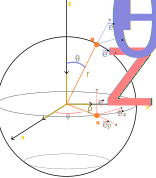
\includegraphics[scale=0.4]{base_s}
\end{multicols}

\subsubsection{Relation entre les vecteurs}
Base cylindrique :
\begin{itemize}
 \item $\vec{e_{\varphi}} = \vec{e_{\varphi}}$
 \item $\vec{e_{r}} = \sin(\theta) \vec{e_{\rho}} + \cos(\theta) \vec{e_z}$
 \item $\vec{e_{\theta}} = \cos(\theta) \vec{e_{\rho}} -\sin(\theta) \vec{e_z}$
\end{itemize}
Base cartésienne :
\begin{itemize}
 \item $\vec{e_{\varphi}} = -\sin(\varphi)\vec{e_x} + \cos(\varphi)\vec{e_y}$
 \item $\vec{e_{r}} = \sin(\theta)\cos(\varphi) \vec{e_x} + \sin(\theta)\sin(\varphi) \vec{e_y}+\cos(\theta)\vec{e_z}$
 \item $\vec{e_{\theta}} = \cos(\theta)\cos(\varphi) \vec{e_x} +\cos(\theta)\sin(\varphi) \vec{e_y} - \sin(\theta)\vec{e_z}$
\end{itemize}
% \subsubsection{Definitions}
% \begin{itemize}
% \item Colatitude : $\theta = \frac{\pi}{2} - \theta_{terrestre}$
% \item p
% \end{itemize}
\section{Cinématique en coordonnées cylindriques}
On considère le temps comme absolu et universel dans tout l'espace. Le temps ne dépend pas de la position. On reste dans la cadre de la physique classique.

On utilise la vitesse instantannée $\vec{V} = \frac{\dd}{\dd t}\vec{OM}$

\subsection{Vecteur position}
$\vec{OM} = \rho \vec{e_{\rho}} + z\vec{e_z}$
\subsection{Vecteur vitesse}
\begin{multicols}{2}
\begin{flalign*}
\vec{v} &= \frac{d\vec{OM}}{dt}\\
&= \frac{d}{dt}(\rho \vec{e_{\rho}})\\
&= \frac{d\rho}{dt}\vec{e_{\rho}}+\rho {\color{red}\frac{d\vec{e_{\rho}}}{dt}}
\end{flalign*}
\columnbreak
\begin{flalign*}
{\color{red}\frac{d\vec{e_{\rho}}}{dt}} &= \frac{d}{dt}(\cos\varphi \vec{e_x} + \sin \varphi \vec{e_y})\\
&= -\frac{d\varphi}{dt}\sin\varphi \vec{e_x}+\frac{d\varphi}{dt}\cos\varphi \vec{e_y}\\
&= \frac{d\varphi}{dt}(-\sin\varphi\vec{e_x}+\cos\varphi\vec{e_y})\\
&= \dot{\varphi}(-\sin\varphi\vec{e_x}+\cos\varphi\vec{e_y})\\
&= {\color{red}\dot{\varphi}(\vec{e_{\varphi}})}
\end{flalign*}
\end{multicols}
\begin{theorem}[Vitesse en coordonnées polaire]
$\vec{v} = \dot{\rho}\vec{e_{\rho}}+\rho\dot{\varphi}\vec{e_{\varphi}} + \dot{z}\vec{e_z}$
\end{theorem}


\subsection{Vecteur accélération en polaire}
\begin{flalign*}
\frac{d\vec{e_{\varphi}}}{dt} &= \frac{d}{dt}(-\sin( \varphi) \vec{e_x}+\cos( \varphi) \vec{e_y})\\
&= -\cos(\varphi)\times\frac{d\varphi}{dt}\vec{e_x} - \sin(\varphi)\frac{d\varphi}{dt}\vec{e_y}\\
&= -\dot{\varphi}(\cos(\varphi)\vec{e_x}+\sin(\varphi)\vec{e_y})\\
&= -\dot{\varphi}\vec{e_{\rho}}
\end{flalign*}
On dérive $\vec{v}$\
\begin{flalign*}
\frac{d\vec{v}}{dt} &= \frac{d}{dt}({\color{orange}\dot{\rho}\vec{e_{\rho}}} + {\color{red}\rho\dot{\varphi}\vec{e_{\varphi}}})\\
&= {\color{orange}\ddot{\rho}\vec{e_{\rho}} + \dot{\rho} \frac{d\vec{e_{\rho}}}{dt}} + {\color{red}\dot{\rho}\dot{\varphi}\vec{e_{\varphi}}+\rho\ddot{\varphi}\vec{e_{\varphi}} + \rho\dot{\varphi}\frac{d\vec{e_{\varphi}}}{dt}}\\
&= {\color{orange}\ddot{\rho}}\vec{e_{\rho}} + {\color{red}\dot{\rho} \dot{\varphi}}(\vec{e_{\varphi}}) +{\color{red}\dot{\rho} \dot{\varphi}}\vec{e_{\varphi}}+{\color{purple}\rho\ddot{\varphi}}\vec{e_{\varphi}} + \rho\dot{\varphi} (-\dot{\varphi})\vec{e_{\rho}}\\
&= ({\color{orange}\ddot{\rho}}-\rho\dot{\varphi}^2)\vec{e_{\rho}}+({\color{purple}\rho\ddot{\varphi}}+2{\color{red}\dot{\rho} \dot{\varphi}})\vec{e_{\varphi}}\\
\end{flalign*}
\begin{theorem}[accélération en coordonnées cylindriques]
\[\vec{a} =  (\ddot{\rho}-\rho\dot{\varphi}^2)\vec{e_{\rho}}+(\rho\ddot{\varphi}+2\dot{\rho}\dot{\varphi})\vec{e_{\varphi}} + \ddot{z}\vec{e_z}\]
\end{theorem}
\section{Cinématique en coordonnées sphériques}
vecteur position : $\vec{OM} = r\vec{e_r}$

vecteur vitesse : $\vec{v} = \dot{r}\vec{e_r}+r\dot{\theta}\vec{e_{\theta}}+r\sin\theta \dot{\varphi}\vec{e_{\varphi}}$.

% vecteur accélération : $(\ddot{r}-r\dot{\theta}^2-r\dot{\varphi}^2\sin(\theta)^2)\vec{e_r}$
\section{Dynamique en base de Frenet}
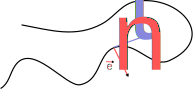
\includegraphics[scale=0.4]{frenet}

Base de l'espace en 2D. On introduit :
\begin{itemize}
 \item $\vec{e_t}$, unitaire et tangent à la trajectoire et dans le sens du mouvement : $\frac{\vec{v}}{\norm{v}}$
 \item $\vec{e_n}$, orthogonal à $\vec{e_t}$. Il est dirigé vers l'intérieur de la concavité.
 \item On peut ajouter un troisème vecteur $\vec{e_b}$ tel que les 3 forment une BOND
\end{itemize}
Vecteur vitesse : $\vec{v} = v\vec{e_t}$

Vecteur accélération : $\vec{a} = \ddot{S}\vec{e_t}+\dot{s}\frac{\dd \vec{e_t}}{\dd t} = \ddot{S}\vec{e_t} + \frac{v^2}{R}\vec{e_n}$, avec $R$ le rayon de courbure.

\warningInfo{Remarque}{Pour un mouvement circulaire, dans la base polaire et de frenet, le vecteur $\vec{e_r}$ est opposé à $\vec{e_{\rho}}$.}
\end{document}
